\chapter{Formation Path-Following Control of 6DOF Underactuated AUVs}
\label{chap:NSB_R}

This chapter presents a method for formation path following control of a fleet of underactuated autonomous underwater vehicles.
The proposed method combines several hierarchic tasks in a \acrlong{nsb} algorithm to safely guide the vehicles.
Compared to the existing literature, the algorithm includes both inter-vehicle and obstacle collision avoidance, and employs a scheme that keeps the vehicles within given operation limits.
The algorithm is applied to a six degree-of-freedom model, using rotation matrices to describe the attitude to avoid singularities.
Using the results of cascaded systems theory, we prove that the closed-loop system is \acrlongpl{usges}.
We use numerical simulations to validate the results.
The contents of this chapter are based on \cite{matous_singularity_2023}.

The chapter is organized as follows.
Section~\ref{sec:NSB_R_problem} introduces the model of the \glspl{auv} and defines the formation path-following problem.
Section~\ref{sec:NSB_R_control} describes the proposed modified \gls{nsb} algorithm.
The stability of the closed-loop system is proven in Section~\ref{sec:NSB_R_path_stability}.
Finally, Section~\ref{sec:NSB_R_simulation} presents the results of the numerical simulations.

\section{Problem Definition}
\label{sec:NSB_R_problem}
In this section, we briefly present the \gls{auv} model and the formation path-following problem.

\subsection{Vehicle Model}
We consider a fleet of $N$ underactuated \glspl{auv}.
The dynamics of the \glspl{auv} are described using the 6\gls{dof} control-oriented model from Section~\ref{sec:model_control_oriented}.
Let $\mat{p} = \inlinevector{x, y, z}$ be the position, and let $\bvel = \inlinevector{u, v, w}$ and $\bs{\omega} = \inlinevector{p, q, r}$ be the linear and angular velocities, respectively.
To avoid the singularities caused by the use of Euler angles, the orientation of the \gls{auv} is given by a rotation matrix $\mat{R} \in SO(3)$.
Furthermore, let $\ocean \in \mathbb{R}^3$ be the velocities of an unknown, constant and irrotational ocean current.

Recalling \eqref{eq:background_nu_dot_relative}, the dynamics of the \glspl{auv} are
\begin{subequations}
\begin{align}
    \dot{\mat{p}} &= \mat{R} \bvel, \label{eq:NSB_R_p_dot}\\
    \dot{\mat{R}} &= \mat{R} \mat{S}(\bs{\omega}), \label{eq:NSB_R_R_dot} \\
    \mat{M} \dot{\vel}_r
        + \bigl(\mat{C}(\vel_r) + \mat{D}(\vel_r)\bigr) \vel_r + \mat{g}(\mat{R}) &= \mat{B}\mat{f}. \label{eq:NSB_R_nu_dot}
\end{align} \label{eq:NSB_R_matrix_vector_model}
\end{subequations}

The aim of this chapter is to demonstrate that the proposed formation path-following algorithm can be readily implemented on vehicles with existing low-level controllers.
Consequently, the choice of a low-level velocity and attitude controller is not discussed in this chapter.
However, there are some assumptions about the low-level controller.

\begin{asm}
    \label{ass5}
    The vehicle is equipped with a low-level controller that allows exponential tracking of the surge velocity, orientation, and angular velocity.
    Specifically, let $u_d, \mat{R}_d$ and $\bs{\omega}_d$ be the reference signals.
    We define an error 
    \begin{align}
        \widetilde{\mat{X}} &= \inlinevector{u - u_d, {\rm logm}\bigl(\widetilde{\mat{R}}\bigr), \bs{\omega} - \widetilde{\mat{R}}\T\bs{\omega}_d}, &
        \widetilde{\mat{R}} &= \mat{R}_d\T\mat{R}, \label{eq:NSB_R_low_level_error}
    \end{align}
    where ${\rm logm} : SO(3) \mapsto \mathbb{R}^3$ is the matrix logarithm \cite{iserles_lie_2000}.
    Note that by Assumption~\ref{asm:actuators}, $\widetilde{\mat{X}}$ is controllable through the input $\mat{f}$.
    Consider the closed-loop system 
    \begin{equation}
        \dot{\widetilde{\mat{X}}} = F \left( \widetilde{\mat{X}}, v, w, \ocean \right), \label{eq:NSB_R_low_level_closed_loop}
    \end{equation}
    consisting of \eqref{eq:NSB_R_R_dot}, \eqref{eq:NSB_R_nu_dot}, and the low-level controller.
    We assume that $\widetilde{\mat{X}} = \mat{0}$ is a \acrfull{ges} equilibrium of \eqref{eq:NSB_R_low_level_closed_loop}.
\end{asm}

An example of a global exponential attitude tracking controller can be found, \emph{e.g.,} in \cite{lee_global_2015}.

Note that for a complete system analysis, we need to consider the underactuated sway and heave dynamics explicitly. 
Recalling \eqref{eq:background_component_form}, the underactuated dynamics have the following form 
\begin{subequations}
    \begin{align}
        \dot{v}_r &= X_v(u_r)r + Y_v(u_r)v_r + Z_v(p)w_r, \\
        \dot{w}_r &= X_w(u_r)q + Y_w(u_r)w_r + Z_w(p)v_r,
        \label{eq:NSB_R_underactuated_dynamics}
    \end{align}
\end{subequations}
where $X(\cdot), Y(\cdot), Z(\cdot)$ are affine functions of the respective variables.

\subsection{Formation Path Following Problem}
\label{sec:NSB_R_objectives}

Similarly to the previous chapter, the goal is to control a fleet of $N$ \glspl{auv} so that they move in a prescribed formation and their barycenter follows a given path.

The prescribed path is parametrized by a smooth function $\mat{p}_p: \mathbb{R} \mapsto \mathbb{R}^3$.
We assume that the function is $\mathcal{C}^{\infty}$ and regular.
Therefore, for every point $\mat{p}_p(s)$ on the path, there exists a path-tangential coordinate frame and a corresponding rotation matrix $\mat{R}_p$ (see Section~\ref{sec:background_paths}).

The path-following error $\mat{p}_b^p$ is given by the position of the barycenter in the path-tangential coordinate frame 
\begin{align}
    \mat{p}_b^p &= \mat{R}_p\T \, \big(\mat{p}_b - \mat{p}_p(s)\big), &
    \mat{p}_b &= \frac{1}{n} \sum_{i=1}^n \mat{p}_i.
    \label{eq:NSB_R_barycenter}
\end{align}
The goal of path following is to control the vehicles so that $\mat{p}_b^p \rightarrow \mat{0}_3$.

The vehicles should converge to a dynamic formation that rotates with the desired path (see Section~\ref{sec:background_formation_keeping} for details).
Let $\mat{p}_{f,1}^f, \ldots, \mat{p}_{f,n}^f$ be the position vectors that represent the desired formation.
The objective is to control the vehicles so that
\begin{align}
    \mat{p}_i - \mat{p}_b &\rightarrow \mat{R}_p(s) \mat{p}_{f,i}^f + \mat{p}_b, &
    i &\in \left\{1, \ldots, n \right\}.
\end{align}

\section{The Proposed Algorithm}
\label{sec:NSB_R_control}

The \glspl{auv} must perform the goals stated in Section \ref{sec:NSB_R_objectives} safely, \emph{i.e.},
avoid collisions with other vehicles and obstacles, and remain within a given range of depths.
An upper limit on the depth of the \glspl{auv} is needed to prevent them from colliding with the seabed or exceeding their depth rating.
A lower limit is needed in busy environments (\emph{e.g.,} harbors), where the \glspl{auv} may otherwise collide or interfere with surface vessels.

To solve the formation path following problem, we propose a method that combines inter-vehicle \acrfull{colav}, formation keeping, \acrfull{los} path following, obstacle avoidance, and depth limiting in a hierarchic manner using an \gls{nsb} algorithm.
Since the \gls{nsb} algorithm outputs inertial velocity references, we also need a method for converting these to surge and orientation.

In this section, we first present the \gls{nsb} algorithm and the associated tasks.
We then present in Section~\ref{sec:NSB_R_references} a strategy for converting inertial velocity references to surge/orientation ones.

\subsection{NSB Algorithm}
\label{sec:NSB_R_NSB}

Similarly to the previous chapter, we define three tasks: \gls{colav}, formation-keeping, and path-following.
Each task will be described in detail in Sections~\ref{sec:NSB_R_COLAV}, \ref{sec:NSB_R_formation}, and \ref{sec:NSB_R_LOS}.
As we will explain in Section \ref{sec:NSB_R_OA}, obstacle avoidance and depth limiting will not be defined as separate tasks but rather achieved through a modification to the path-following task.
Let us denote the variables associated with the \gls{colav}, formation-keeping, and path-following tasks by lower indices $1$, $2$, and $3$, respectively.
Define the so-called \emph{task variables} as $\bs{\sigma}_i = \bs{f}_i\left(\mat{p}_1, \ldots, \mat{p}_n\right), i \in \left\{1,2,3\right\}$, and their desired values as $\bs{\sigma}_{d,i}, i \in \left\{1,2,3\right\}$.

Furthermore, let $\ivel_i, i \in \left\{1,2,3\right\}$ be the desired velocities of each task.    
These velocities are combined using the recursive \gls{nsb} algorithm \eqref{eq:background_NSB_recursive}.
\begin{equation} 
    \ivel_{\rm NSB} = \ivel_1 + \mat{N}_1\left(\ivel_2 + \mat{N}_2\ivel_3\right). \label{eq:NSB_R_NSB_with_COLAV}
\end{equation}

\subsection{Inter-Vehicle Collision Avoidance}
\label{sec:NSB_R_COLAV}

Let {$d_{\rm COLAV}$} be the \emph{activation distance}, \emph{i.e.,} the distance at which the vehicles need to start performing the evasive maneuvers.
The task variable is given by a vector of relative distances between the vehicles smaller than $d_{\rm COLAV}$
\begin{align}
        \bs{\sigma}_1 &= \big[\norm{\mat{p}_i - \mat{p}_j}\big], &
        \begin{split} 
            \forall &i,j\in\{1,\ldots,n\}, j > i, \\
            &\norm{\mat{p}_i - \mat{p}_j} < d_{\rm COLAV}.
        \end{split}
\end{align}
The desired values of the task are 
\begin{equation}
    \bs{\sigma}_{d,1} = d_{\rm COLAV} \, \mat{1},
\end{equation}
where $\mat{1}$ is a vector of ones.
To ensure a faster response to a potential collision than in the previous chapter, we propose the following sliding-mode-like \gls{colav} velocity 
\begin{align}
    \ivel_1 &= - U_{\rm COLAV} \mat{J}_1^{\dagger} \frac{\widetilde{\bs{\sigma}}_1}{\norm{\widetilde{\bs{\sigma}}_1}}, &
    \widetilde{\bs{\sigma}}_1 &= \bs{\sigma}_1 - \bs{\sigma}_{d, 1},
\end{align}
where $U_{\rm COLAV}$ is a positive constant.

Similarly to the previous chapter, this task does not guarantee robust collision avoidance.
During the transients, the relative distance may become smaller than $d_{\rm COLAV}$.
Therefore, to ensure collision avoidance, $d_{\rm COLAV}$ should be chosen as $d_{\rm min} + d_{\rm sec}$, where $d_{\rm min}$ is the minimum safe distance between the vehicles, and $d_{\rm sec}$ is an additional security distance.

\subsection{Formation Keeping}
\label{sec:NSB_R_formation}
The formation-keeping task variable is defined as
\begin{align}
    \bs{\sigma}_2 &= \inlinevector{\bs{\sigma}_{2,1}, \ldots, \bs{\sigma}_{2,n-1}}, \label{eq:NSB_R_sigma_2} &
    \bs{\sigma}_{2,i} &= \mat{p}_i - \mat{p}_b,
\end{align}
and its desired values are 
\begin{equation}
    \bs{\sigma}_{d,2} = \inlinevector{\mat{R}_p\,\mat{p}_{f,1}^f, \ldots, \mat{R}_p\,\mat{p}_{f,n-1}^f}  .
    \label{eq:NSB_R_sigma_d_2}
\end{equation}
%Similarly to \gls{colav}, we use the CLIK equation~\eqref{eq:NSB_R_CLIK} to obtain the formation-keeping velocity.
%However, as motivated in Section~\ref{sec:NSB_R_references}, this velocity needs to be saturated.
The formation-keeping velocity is given by 
\begin{align}
    \ivel_2 &= \mat{J}_2^{\dagger}\dot{\bs{\sigma}}_{d,2} - \ivels_{2, \max}\mat{J}_2^{\dagger}\,{\rm sat}\left(\bs{\Lambda}_2\widetilde{\bs{\sigma}}_2\right), &
    \widetilde{\bs{\sigma}}_2 &= \bs{\sigma}_2 - \bs{\sigma}_{d, 2},
    \label{eq:NSB_R_v_form}
\end{align}
where $\ivels_{2, \max}$ is a positive constant, and $\rm sat$ is a saturation function given by 
\begin{equation}
    {\rm sat}(\mat{x}) = \mat{x} \frac{{\rm tanh}\left(\norm{\mat{x}}\right)}{\norm{\mat{x}}}.
\end{equation}
The use of a saturation function guarantees some bounds on the \gls{nsb} velocity, as we will explain in Section~\ref{sec:NSB_R_references}.

\subsection{Path Following}
\label{sec:NSB_R_LOS}

To solve the path-following, we employ the coupled \gls{los} guidance algorithm \eqref{eq:background_los_coupled}.
Let $\Delta\left(\mat{p}_b^p\right)$ be the lookahead distance of the LOS guidance law.
Inspired by \cite{belleter_2019_observer}, we choose an error-dependent lookahead distance 
\begin{equation}
    \Delta\left(\mat{p}_b^p\right) = \sqrt{\Delta_0^2 + \left(x_b^p\right)^2 + \left(y_b^p\right)^2 + \left(z_b^p\right)^2}
    \label{eq:NSB_R_delta}
\end{equation}
where $\Delta_0$ is a positive constant.
The LOS velocity then is 
\begin{equation}
    \ivel_{\rm LOS} = \frac{U_{\rm LOS}}{D} \, \mat{R}_p\inlinevector{\Delta\left(\mat{p}_b^p\right), -y_b^p, -z_b^p},
    \label{eq:NSB_R_v_LOS}
\end{equation}
where $U_{\rm LOS} > 0$ is the desired path-following speed, and 
\begin{equation}
    D = \sqrt{\Delta(\cdot)^2 + \left(y_b^p\right)^2 + \left(z_b^p\right)^2}.
\end{equation}
The task velocity is then given by 
\begin{equation}
    \ivel_3 = \mat{1}_N \otimes \ivel_{\rm LOS}.
    \label{eq:NSB_R_v_3}
\end{equation}

Note that the path parameter $s$ in~\eqref{eq:NSB_R_barycenter} can be treated as an additional degree of freedom in the control design, and used to get a stable behavior of the along-track error $x_b^p$. 
Inspired by \cite{belleter_2019_observer}, we choose the update law of $s$ as
\begin{equation}
    \dot{s} = \norm{\frac{\partial \mat{p}_p(s)}{\partial s}}^{-1} U_{\rm LOS} \left(\frac{\Delta}{D} + k_{s}\,\frac{x_b^p}{\sqrt{1+\left(x_b^p\right)^2}}\right),\label{eq:NSB_R_path_update}
\end{equation}
where $k_{s}$ is a positive gain.
% Damiano: maybe we should also say something along "other choices could have been possible, e.g., by taking inspiration from X Y Z, but our experience seems to indicate that the final performance is not too much affected by this choice"? 


\subsection{Obstacle Avoidance and Depth Limiting}
\label{sec:NSB_R_OA}

Obstacle avoidance is typically implemented individually for each vehicle \cite{antonelli_2006_kinematic}.
However, we propose to perform this task globally by incorporating it into the path-following algorithm so that it does not interfere with the inter-vehicle \gls{colav}. %(indeed, inter-vehicle \gls{colav} may be ensured by changing opportunely the relative velocities of the vehicles).

To arrive at the proposed algorithm, we first restrict the obstacle avoidance maneuvers to the $xy$-plane to avoid interfering with the subsequent depth-limiting logic.
Let $\mat{p}_o = \inlinevector{x_o, y_o, z_o}$ be the position of the obstacle and $r_o$ the obstacle avoidance radius.
Note that $r_o$ must be chosen sufficiently large to cover the size of both the obstacle and the \gls{auv}. %(and relative uncertainties).
Furthermore, let us define the formation radius
$
    r_f = \max_{i \in \{1, \ldots, n\}} \norm{\inlinevector{x_b-x_i, y_b-y_i}}
$
and the relative position $\mat{p}_{\rm rel} = \inlinevector{x_b - x_o, y_b - y_o}$. As illustrated in \figref{fig:NSB_R_obstacle_radius}, obstacle avoidance is ensured if 
\begin{equation}
    \norm{\mat{p}_{\rm rel}} \geq r_o + r_f. \label{eq:NSB_R_obstacle_avoidance_condition}
\end{equation}

\begin{figure}[t]
    \centering
    \begin{subfigure}[t]{0.33\textwidth}
        \centering
        \def\svgwidth{\textwidth}
        \import{figures/nsb_R}{obstacle_avoidance.pdf_tex}
        \vspace*{-0.25em}
        \caption{Obstacle and formation radii}
        \label{fig:NSB_R_obstacle_radius}
        \vspace*{-0.25em}
    \end{subfigure}   
    \begin{subfigure}[t]{0.33\textwidth}
        \centering
        \def\svgwidth{\textwidth}
        \import{figures/nsb_R}{collision_cone.pdf_tex}
        \vspace*{-0.25em}
        \caption{Collision cone}
        \label{fig:NSB_R_collision_cone}
        \vspace*{-0.25em}
    \end{subfigure} 
    \caption{Illustration motivating the obstacle avoidance constraint~\eqref{eq:NSB_R_obstacle_avoidance_condition} and conflict condition~\eqref{eq:NSB_R_collision-conflict}.}     
    
\end{figure}



To guarantee obstacle avoidance, we utilize the collision cone concept \cite{chakravarthy_obstacle_1998}. 
Inspired by \cite{wiig_collision_2019}, we employ a constant avoidance angle and define a switching condition.
More precisely, let 
\begin{equation}
    \ivel_{\rm rel} = \inlinevector{\ivels_{x, {\rm LOS}} - \dot{x}_o, \ivels_{y, {\rm LOS}} - \dot{y}_o}
    \label{eq:NSB_R_v_rel}
\end{equation}
denote the relative line-of-sight velocity ($\ivels_{x, {\rm LOS}}$ and $\ivels_{y, {\rm LOS}}$ are the components of $\ivel_{\rm LOS}$).
As shown in~\figref{fig:NSB_R_collision_cone}, a conflict between the \glspl{auv} and the obstacle arises if the relative velocity lies in the so-called \emph{collision cone}, \emph{i.e.}, if
\begin{align}
    \abs{\angle\left(\mat{p}_{\rm rel}, -\ivel_{\rm rel}\right)} &\leq \alpha, &
    \alpha &= \sin^{-1}\left(\frac{r_o+r_f}{\norm{\mat{p}_{\rm rel}}}\right),
    \label{eq:NSB_R_collision-conflict}
\end{align}
where $\angle\left(\mat{a}, \mat{b}\right)$ denotes the angle between two vectors.


The obstacle avoidance task is activated if simultaneously such a conflict arises and the cone angle satisfies 
$\alpha \geq \alpha_{\min}$, where $0 < \alpha_{\min} \ll \pi / 2$.
Note that \cite{wiig_collision_2019} use a switching condition based on distance, \emph{i.e.,}
$\norm{\mat{p}_{\rm rel}} \leq d_{\min}$.
Since our definition of a safe distance \eqref{eq:NSB_R_obstacle_avoidance_condition} is not constant, we instead suggest using a switching rule based on the cone angle.



When the task is active, the $x$- and $y$-components of the LOS velocity are replaced by the obstacle avoidance velocity $\ivel_{\rm OA}$ given by 
\begin{align}
    \ivel_{\rm OA} &= \norm{\ivel_{\rm rel}} \inlinevector{\cos(\psi_{\rm OA}), \sin(\psi_{\rm OA})} + \inlinevector{\dot{x}_o, \dot{y}_o}, \\
    \psi_{\rm OA} &= {\rm atan}_2 \left(y_o - y_b, x_o - x_b\right) \pm \alpha.
\end{align}
Note that $\psi_{\rm OA}$ has two solutions corresponding to the clockwise and counterclockwise directions.
Inspired by \cite{haraldsen_reactive_2021}, we propose the following method for choosing a direction:
When the conflict first happens, we choose the value of $\psi_{\rm OA}$ that is closer to the direction of $\ivel_{\rm rel}$.
Afterwards, we maintain the same direction.



As for the depth-limiting logic,
let $z_{\min}$ and $z_{\max}$ be the operation limits.
We assume the limits to be wide enough to accommodate the formation.
We then propose to replace the $z$-component of the LOS velocity with a depth-limiting velocity $\ivels_{z, {\rm lim}}$ given by 
\begin{equation}
    \ivels_{z, {\rm lim}} = \begin{cases}
        \ivels_z, & \text{if } \min_{i \in \{1, \ldots, n\}} z_i \leq z_{\min}, \\
        -\ivels_z, & \text{if } \max_{i \in \{1, \ldots, n\}} z_i \geq z_{\max}, \\
        \ivels_{z, {\rm LOS}}, & \text{otherwise},
    \end{cases}
\end{equation}
where $\ivels_z$ is a positive constant.


\subsection{Surge and Orientation References}
\label{sec:NSB_R_references}

Since the \gls{nsb} algorithm outputs inertial velocity references, we also need a method for converting these to surge and orientation references.
The strategy for choosing these references changes depending on whether the avoidance or depth-limiting tasks are active.
The proposed strategy allows us to prove the closed-loop stability of both the path-following and formation-keeping tasks (\emph{c.f.} \cite{arrichiello_formation_2006}, where no stability proofs are given, and \cite{eek_formation_2021,matouvs_formation_2022}, that only prove the stability of the path-following task).



First, let us consider the case when neither the avoidance nor depth-limiting tasks are active.
Because the formation-keeping and the path-following task are independent and orthogonal, \eqref{eq:NSB_R_NSB_with_COLAV} can be simplified to 
\begin{equation}
    \ivel_{\rm NSB} = \ivel_2 + \ivel_3.
    \label{eq:NSB_R_NSB_nominal_simplified}
\end{equation}


\noindent Let $\ivel_{{\rm NSB}, i}$ denote the desired velocity of vehicle $i$.    
To achieve the desired behavior, the surge reference $u_{d, i}$ must satisfy 
\begin{equation}
    u_{d, i} = \sqrt{\norm{\ivel_{{\rm NSB}, i}}^2 - v_i^2 - w_i^2},
    \label{eq:NSB_R_surge_reference}
\end{equation}


\noindent However, \eqref{eq:NSB_R_surge_reference} can only be satisfied if 
\begin{equation}
    \norm{\ivel_{{\rm NSB}, i}}^2 \geq v_i^2 + w_i^2.
\end{equation}
In addition, \glspl{auv} typically need to maintain a minimum surge velocity to be able to maneuver, implying a stricter inequality 
\begin{equation}
    \norm{\ivel_{{\rm NSB}, i}}^2 \geq u_{\min}^2 + v_i^2 + w_i^2
    \label{eq:NSB_R_NSB_speed_condition}
\end{equation}
where $u_{\min} > 0$.
This inequality can be satisfied by choosing a time-varying path-following speed $U_{\rm LOS}$.



Substituting task velocity definitions \eqref{eq:NSB_R_v_form} and \eqref{eq:NSB_R_v_3} into \eqref{eq:NSB_R_NSB_nominal_simplified} and exploiting the structure of the task Jacobian $\mat{J}_2$, we get that the \gls{nsb} velocity of vehicle $i$ is given by 
\begin{equation}
    \ivel_{{\rm NSB}, i} = \ivel_{\rm LOS} + \dot{\mat{R}}_p(s)\mat{p}_{f,i}^f + \ivel_{2,i}, \label{eq:NSB_R_v_NSB_i}
    \vspace*{-0.55em}
\end{equation}
where 
\begin{equation}
    \inlinevector{\ivel_{2, 1}, \ldots, \ivel_{2, n}} = 
    - \ivels_{2, \max}\,{\rm sat}\left(\mat{J}_2^{\dagger}\bs{\Lambda}_2 \widetilde{\bs{\sigma}}_2\right). \label{eq:NSB_R_v_form_components}
\end{equation}
Let $\bs{\omega}_p(s)$ be a vector such that 
\begin{equation}
    \dot{\mat{R}}_p(s) = \mat{R}_p(s)\,\mat{S}\bigl(\bs{\omega}_p(s)\bigr)\,\dot{s}. \label{eq:NSB_R_R_p_dot}
\end{equation}
\eqref{eq:NSB_R_path_update} implies the following upper bound 
\begin{equation}
    \abs{\dot{s}} \leq \norm{\frac{\partial \mat{p}_p(s)}{\partial s}}^{-1} U_{\rm LOS} \left(1 + k_{s}\right). \label{eq:NSB_R_path_update_bound}
\end{equation}
Substituting \eqref{eq:NSB_R_v_form_components}, \eqref{eq:NSB_R_R_p_dot}, and \eqref{eq:NSB_R_path_update_bound} into \eqref{eq:NSB_R_v_NSB_i}, we get the following lower bound on the \gls{nsb} velocity 
\begin{equation}
    \norm{\ivel_{{\rm NSB}, i}} \geq U_{\rm LOS} \left(1
        - \norm{\bs{\omega}_p}\norm{\scale[1]{\frac{\partial \mat{p}_p}{\partial s}}}^{-1}\norm{\mat{p}_{f, i}^f} \left(1 + k_{s}\right)\right) - \ivels_{2, \max}.
\end{equation}
Now, assuming the existence of an upper bound on the product $$\norm{\bs{\omega}_p(s)}\norm{\partial \mat{p}_p(s) / \partial s}^{-1},$$ there exists a positive constant $k_{\rm NSB}$ such that for every vehicle 
\begin{equation}
    \norm{\ivel_{{\rm NSB}, i}} \geq (1 - k_{\rm NSB})U_{\rm LOS} - \ivels_{2, \max}.
\end{equation}
Assuming that $k_{\rm NSB} < 1$, we can satisfy \eqref{eq:NSB_R_NSB_speed_condition} by choosing 
\begin{equation}
    U_{\rm LOS} = \frac{\ivels_{2, \max} + \max_i \sqrt{v_i^2 + w_i^2 + u_{\min}^2}}{1 - k_{\rm NSB}}.
\end{equation}
However, the $\max$ function would introduce switching behavior.
To avoid this, we approximate the former with 
\begin{equation}
    U_{\rm LOS} = \frac{\ivels_{2, \max} + \sqrt{\sum_{i=1}^n \left(v_i^2 + w_i^2\right) + u_{\min}^2}}{1 - k_{\rm NSB}}.
    \label{eq:NSB_R_U_LOS}
\end{equation}


If the avoidance or depth-limiting tasks are active, we still choose $U_{\rm LOS}$ in accordance with \eqref{eq:NSB_R_U_LOS}.
However, since \eqref{eq:NSB_R_NSB_speed_condition} cannot be satisfied with a generic \gls{nsb} velocity \eqref{eq:NSB_R_NSB_with_COLAV}, we choose the surge reference as 
\begin{equation}
    u_{d, i} = 
    \begin{cases}
        \sqrt{\norm{\ivel_{{\rm NSB}, i}}^2 - v_i^2 - w_i^2},  &\text{if \eqref{eq:NSB_R_NSB_speed_condition} satisfied,} \\
        u_{\rm min}, &\text{otherwise}.
    \end{cases}
\end{equation}


Finally, let us discuss the choice of desired orientation.
Let $\overline{\ivel}_{{\rm NSB}, i}$ and $\overline{\bvel}_{i}$ denote normalized vectors.
We are seeking $\mat{R}_{d, i} \in SO(3)$ such that 
\begin{equation}
    \overline{\ivel}_{{\rm NSB}, i} = \mat{R}_{d, i}\,\overline{\bvel}_{i}.
    \label{eq:NSB_R_rotation_reference}
\end{equation}
Assume that at a given time, there is $\mat{R}_{d, i}$ that satisfies \eqref{eq:NSB_R_rotation_reference}.
Differentiating \eqref{eq:NSB_R_rotation_reference} with respect to time yields 
\begin{equation}
    \dot{\overline{\ivel}}_{{\rm NSB}, i} = \mat{R}_{d, i}\,\mat{S}(\bs{\omega}_{d, i})\,\overline{\bvel}_{i} + \mat{R}_{d, i}\,\dot{\overline{\bvel}}_{i},
    \label{eq:NSB_R_rotation_reference_derivative1}
\end{equation}
where $\bs{\omega}_{d, i}$ is the desired angular velocity of the vehicle.     
Let us define
\begin{align}
    \bs{\omega}_{\ivel_{{\rm NSB}, i}} &= \overline{\ivel}_{{\rm NSB}, i} \times \dot{\overline{\ivel}}_{{\rm NSB}, i}, &
    \bs{\omega}_{\bvel_{i}} &= \overline{\bvel}_{i} \times \dot{\overline{\bvel}}_{i}.
    \label{eq:NSB_R_omega_v}
\end{align}    
Then, \eqref{eq:NSB_R_rotation_reference_derivative1} can be rewritten as 
\begin{equation}
    \bs{\omega}_{\ivel_{{\rm NSB}, i}} \times \overline{\ivel}_{{\rm NSB}, i} = 
    \mat{R}_{d, i} \left( \bs{\omega}_{d, i} \times \overline{\bvel}_{i} + \bs{\omega}_{\bvel_{i}} \times \overline{\bvel}_{i} \right).
\end{equation}
Therefore, the desired angular velocity must satisfy 
\begin{equation}
    \left( \bs{\omega}_{d, i} + \bs{\omega}_{\bvel_{i}} 
    - \mat{R}_{d, i}\T \bs{\omega}_{\ivel_{{\rm NSB}, i}} \right) \times \overline{\bvel}_{i} = \mat{0}. \label{eq:NSB_R_omega_ref_equation}
\end{equation}
Thus, instead of finding $\mat{R}_{d, i}$ directly, we propose to choose 
\begin{equation}
    \bs{\omega}_{d, i} = \mat{R}_{d, i}\T \bs{\omega}_{\ivel_{{\rm NSB}, i}} - \bs{\omega}_{\bvel_{i}},
    \label{eq:NSB_R_omega_ref}
\end{equation}
and then evolve the desired orientation according to 
\begin{equation}
    \dot{\mat{R}}_{d, i} = \mat{R}_{d, i} \mat{S}(\bs{\omega}_{d, i}).
\end{equation}
Note that choosing $\bs{\omega}_{d, i}$ according to \eqref{eq:NSB_R_omega_ref} leads to the smallest (in terms of Euclidean norm) angular velocity that satisfies \eqref{eq:NSB_R_omega_ref_equation}.
We also note that there exists a subspace of angular velocities that satisfy \eqref{eq:NSB_R_omega_ref_equation} and a subspace of rotation matrices that satisfy \eqref{eq:NSB_R_rotation_reference}.
This differs from 3\gls{dof} \cite{eek_formation_2021,arrichiello_formation_2006} and 5\gls{dof} \cite{matouvs_formation_2022} models, for which only one solution exists.


\section{Closed-Loop Analysis}
\label{sec:NSB_R_path_stability}

In this section, we analyze the closed-loop behavior of the system.
Throughout this section, we assume that neither the avoidance nor depth-limiting tasks are active.
Let us define the combined formation-keeping and path-following error as 
\begin{equation}
    \widetilde{\bs{\sigma}} = \inlinevector{\widetilde{\bs{\sigma}}_2, \left(\mat{p}_b^p\right)},
\end{equation}
and the combined low-level controller error as
\begin{equation}
    \widetilde{\mat{X}} = \inlinevector{\widetilde{\mat{X}}_1, \ldots, \widetilde{\mat{X}}_n}.
\end{equation}
First, let us investigate the closed-loop dynamics of $\widetilde{\bs{\sigma}}$.
Differentiating \eqref{eq:NSB_R_sigma_2}, \eqref{eq:NSB_R_sigma_d_2}, and \eqref{eq:NSB_R_barycenter} with respect to time yields 
\begin{subequations}
\begin{align}
    \dot{\widetilde{\bs{\sigma}}}_2 &= \mat{J}_2\dot{\mat{p}} - \dot{\bs{\sigma}}_{d, 2}, \qquad \dot{\mat{p}} = \inlinevector{\dot{\mat{p}}_1, \ldots, \dot{\mat{p}}_n} \\
    \dot{\mat{p}}_b^p &= \mat{R}_p\T\left(\frac{1}{n}\sum_{i=1}^n\dot{\mat{p}}_i - \dot{\mat{p}}_p\right) - \mat{S}\big(\bs{\omega}_p\dot{s}\big)\mat{p}_b^p.
\end{align} \label{eq:NSB_R_dot_sigma_tilde}
\end{subequations}
From \eqref{eq:NSB_R_p_dot} and \eqref{eq:NSB_R_low_level_error} it follows that $\dot{\mat{p}}_i$ is given by 
\begin{align}
    \dot{\mat{p}}_i &= \mat{R}_i\bvel_i = {\rm expm}\left(\bs{\delta}_i\right)\mat{R}_{d, i}\inlinevector{u_{d, i} + \widetilde{u}_i, v_i, w_i}, \label{eq:NSB_R_p_dot_closed_loop}
\end{align}
with 
\begin{align}
    {\rm expm}(\bs{\delta}) &= \cos\theta\,\mat{I} + s\mat{S}(\bs{\delta}) + c\mat{S}(\bs{\delta})^2\mathrlap{,} &
    &\begin{array}{l}
    \scale[1]{\theta = \norm{\bs{\delta}},} \\
    \scale[1]{s = \frac{\sin(\theta)}{\theta},} \\
    \scale[1]{c = \frac{1 - \cos(\theta)}{\theta^2}.}
    \end{array} \label{eq:NSB_R_expm}
\end{align}
Substituting \eqref{eq:NSB_R_expm}, \eqref{eq:NSB_R_surge_reference}, and \eqref{eq:NSB_R_rotation_reference} into \eqref{eq:NSB_R_p_dot_closed_loop} we get 
\begin{equation}
    %\begin{split}
    \dot{\mat{p}}_i = \ivel_{{\rm NSB}, i} 
                + s(\bs{\delta}_i \times \ivel_{{\rm NSB}, i})
                + c\,\bs{\delta}_i\times(\bs{\delta}_i \times \ivel_{{\rm NSB}, i})
                + \mat{R}_{i}\inlinevector{\widetilde{u}_i, 0, 0}.
    %\end{split} \label{eq:NSB_R_p_dot_closed_loop_2}
    \label{eq:NSB_R_p_dot_closed_loop_2}
\end{equation}
Defining a perturbing term $\mat{g}_i$ as 
\begin{equation}
    \mat{g}_i = s(\bs{\delta}_i \times \ivel_{{\rm NSB}, i}) 
                + c\,\bs{\delta}_i\times(\bs{\delta}_i \times \ivel_{{\rm NSB}, i}) 
                + \mat{R}_{i}\inlinevector{\widetilde{u}_i, 0, 0},
                \label{eq:NSB_R_g_i}
\end{equation}
and substituting \eqref{eq:NSB_R_g_i} and \eqref{eq:NSB_R_p_dot_closed_loop_2} into \eqref{eq:NSB_R_dot_sigma_tilde} yields 
\begin{subequations}
    \begin{align}
        \dot{\widetilde{\bs{\sigma}}}_2 &= \mat{J}_2\ivel_{\rm NSB} - \dot{\bs{\sigma}}_{d, 2}
                                        +\mat{J}_2\mat{G}, \qquad \mat{G} = \inlinevector{\mat{g}_1, \ldots, \mat{g}_n} \\
        \dot{\mat{p}}_b^p &= \mat{R}_p\T\left(\!\frac{1}{n}\sum_{i=1}^n\left(\ivel_{{\rm NSB}, i} + \mat{g}_i\right) - \dot{\mat{p}}_{\mathrlap{p}}\right) - \mat{S}\big(\bs{\omega}_p\dot{s}\big)\mat{p}_b^p \mathrlap{.}
    \end{align} \label{eq:NSB_R_outer_loop}
\end{subequations}
Now, to account for the underactuated dynamics, we define a vector of concatenated sway and heave velocities as 
\begin{align}
    \bvel_u &= \inlinevector{v_1, w_1, \ldots, v_n, w_n}, &
    \bvel_{u, c} &= \mat{1}_n \otimes \inlinevector{v_c, w_c}.
\end{align}
The underactuated dynamics can then be written as
\begin{equation}
    \dot{\bvel}_u = \mat{X}\bs{\Omega} + \mat{Y}\left(\bvel_u - \bvel_{u, c}\right) + \dot{\bvel}_{u, c}, \label{eq:NSB_R_underactuated_dynamics_closed_loop}
\end{equation}
where $\bs{\Omega} = \inlinevector{\bs{\omega}_1, \ldots, \bs{\omega}_n}$, and $\mat{X}$ and $\mat{Y}$ are block diagonal matrices consisting of blocks $\mat{X}_1, \ldots, \mat{X}$ and $\mat{Y}_1, \ldots, \mat{Y}_n$, that are given by 
\begin{align}
    \mat{X}_i &= 
    \begin{bmatrix}
        0 & 0 & X_v(u_{r, i}) \\
        0 & X_w(u_{r, i}) & 0
    \end{bmatrix}, &
    \mat{Y}_i &=
    \begin{bmatrix}
        Y_v(u_{r,i}) & Z_v(p_i) \\
        Z_w(p_i) & Y_w(u_{r, i})
    \end{bmatrix}.
\end{align}


\begin{theorem} \label{thm_NSB_R}
    Let Assumptions \ref{asm:symmetric}--\ref{ass5} be satisfied.
    Then, $\left[\widetilde{\bs{\sigma}}\T, \widetilde{\bs{X}}\T\right] = \mat{0}\T$ is a \acrfullpl{usges} equilibrium point of the closed-loop system \eqref{eq:NSB_R_outer_loop}, \eqref{eq:NSB_R_low_level_closed_loop}, \eqref{eq:NSB_R_underactuated_dynamics_closed_loop}.
    Moreover, if the second and third partial derivatives of $\mat{p}_p(s)$ with respect to $s$ are bounded and \eqref{eq:NSB_R_boudedness_condition} is satisfied, the underactuated sway and heave dynamics are bounded near the manifold $\left[\widetilde{\bs{\sigma}}, \widetilde{\bs{X}}\right] = \mat{0}\T$.
\end{theorem}

\begin{proof}
    We analyze the closed-loop system as a cascade where $\widetilde{\bs{X}}$ perturbs the dynamics of $\widetilde{\bs{\sigma}}$ through $\mat{G}$.
    Consider the nominal dynamics of $\widetilde{\bs{\sigma}}$ (\emph{i.e.}, \eqref{eq:NSB_R_outer_loop} with $\mat{G} = \mat{0}$) and the following Lyapunov function candidate 
    \begin{equation}
        V = \frac{1}{2}\,\widetilde{\bs{\sigma}}\T\widetilde{\bs{\sigma}} = \frac{1}{2}\left(\widetilde{\bs{\sigma}}_2\T\widetilde{\bs{\sigma}}_2 + \left(\mat{p}_b^p\right)\T\mat{p}_b^p\right).
    \end{equation}
    The time-derivative of $V$ is 
    \begin{equation}
        %\begin{split}
            \dot{V}\! = \widetilde{\bs{\sigma}}_2\T\!\left(\mat{J}_2\ivel_{\rm NSB} - \dot{\bs{\sigma}}_{d, 2}\right)
            - \left(\mat{p}_b^p\right)\T\!\mat{S}\!\left(\bs{\omega}_p\dot{s}\right)\!\mat{p}_b^p 
            + \left(\mat{p}_b^p\right)\T\!\mat{R}_p\T\bigg(\frac{1}{n}\sum_{i=1}^n\ivel_{{\rm NSB}, i} - \dot{p}_p\!\bigg) .
        %\end{split} 
        \label{eq:NSB_R_Lyapunov_analysis_step1}
    \end{equation}
    Due to the properties of the \gls{nsb} tasks defined in Sections \ref{sec:NSB_R_formation} and \ref{sec:NSB_R_LOS}, the following identities hold: 
    \begin{align}
        \mat{J}_2\ivel_{\rm NSB} &= \mat{J}_2\ivel_2, &
        \sum_{i=1}^n \ivel_{{\rm NSB}, i} &= \ivel_{\rm LOS}.
    \end{align}
    By definition (see Section \ref{sec:NSB_R_objectives}), $\mat{R}_p$ must satisfy 
    \begin{align}
        \mat{R}_p\T\dot{p}_p &= \dot{s}\norm{\scale[1]{\frac{\partial \mat{p}_p(s)}{\partial s}}}^{-1}\mat{e}_1, &
        \mat{e}_1 &= \inlinevector{1, 0, 0}.
    \end{align}
    Substituting \eqref{eq:NSB_R_v_form} and \eqref{eq:NSB_R_v_LOS} into \eqref{eq:NSB_R_Lyapunov_analysis_step1} leads to 
    \begin{equation}
        \begin{split}
        \dot{V} &= -\ivels_{2, \rm max} \widetilde{\bs{\sigma}}_2\T {\rm sat}\left(\bs{\Lambda}_2\widetilde{\bs{\sigma}}_2\right) \\
                &\quad -U_{\rm LOS} \scale[1]{\left(
                    k_{s}\frac{\left(x_b^p\right)^2}{\sqrt{1 + \left(x_b^p\right)^2}} +
                    \frac{\left(y_b^p\right)^2}{D} +
                    \frac{\left(z_b^p\right)^2}{D}
                  \right)}.
        \end{split}
        \label{eq:NSB_R_Lyapunov_analysis_step2}
    \end{equation}
    For any $\widetilde{\bs{\sigma}} \in \ball[3N]{r}$, the following holds: 
    \begin{equation}
        \begin{split}
        \dot{V} &\leq  - \ivels_{2, \max}\lambda_{2, \min}\scale[1]{\frac{{\rm tanh}(r)}{r}}\norm{\widetilde{\bs{\sigma}}_2}^2 \\
                &\quad - U_{\rm LOS}\min\left\{\scale[1]{\frac{k_{s}}{\sqrt{1+r^2}}, \frac{1}{\sqrt{\Delta_0^2+2r^2}}}\right\}\norm{\mat{p}_b^p}^2,
        \end{split}
        \label{eq:NSB_R_Lyapunov_analysis_step3}
    \end{equation}
    where $\lambda_{2, \min}$ is the smallest eigenvalue of $\bs{\Lambda}_2$.
    From \eqref{eq:NSB_R_Lyapunov_analysis_step3}, we conclude that the derivative of $V$ satisfies
    \begin{equation}
        \dot{V} \leq - k_r \norm{\widetilde{\bs{\sigma}}}^2,
    \end{equation}
    where
    \begin{equation}
        k_r = \min \left\{\ivels_{2, \max}\lambda_{2, \min}\scale[1]{\frac{{\rm tanh}(r)}{r}}, 
                          \scale[1]{\frac{U_{\rm LOS}k_{s}}{\sqrt{1+r^2}}}, 
                          \scale[1]{\frac{U_{\rm LOS}}{\sqrt{\Delta_0^2+2r^2}}}\right\}
    \end{equation}
    All assumptions of \cite[Theorem 5]{pettersen_lyapunov_2017} are thus satisfied, and the origin of the nominal system is \glspl{usges}.

    

    Moreover, note that the low-level controller is \gls{ges} by Assumption \ref{ass5}.
    Therefore, if the two assumptions of Proposition~\ref{prop:background_cascade} hold, the origin of the cascade is \glspl{usges}.
    Since $\norm{\partial V / \partial \widetilde{\bs{\sigma}}} = \norm{\widetilde{\bs{\sigma}}}$, the first assumption is satisfied for $c_1 = \sfrac{1}{2}$, $c_2 = \eta$, and any $\eta \in \mathbb{R}_{\geq 0}$.    

    To validate the second assumption, we first need to investigate the perturbing terms $\mat{g}_i$ from \eqref{eq:NSB_R_g_i}.
    From \eqref{eq:NSB_R_v_NSB_i} we get the following upper bound on $\ivel_{{\rm NSB}, i}$ 
    \begin{align}
        \norm{\ivel_{{\rm NSB}, i}} &\leq U_{\rm LOS}\left(1 + k_{\rm NSB}\right) + \ivels_{2, \max}\tanh\left(\norm{\widetilde{\bs{\sigma}}_2}\right),
    \end{align}
    and from \eqref{eq:NSB_R_expm}, we get the inequalities 
    \begin{align}
        s &\leq 1, &
        \norm{c\,\bs{\delta}} &\leq \sfrac{\sqrt{2}}{2}.
    \end{align}
    Therefore, $\mat{g}_i$ can be upper-bounded by 
    \begin{equation}
        \norm{\mat{g}_i} \leq \norm{\ivel_{{\rm NSB}, i}}\left(1 + \sfrac{\sqrt{2}}{2}\right)\norm{\bs{\delta}_i} + \abs{\widetilde{u}_i}.
    \end{equation}
    Consider then the two functions $\alpha_{1,i}, \alpha_{2,i} : \mathbb{R}_{\geq 0} \mapsto \mathbb{R}_{\geq 0}$ 
    \begin{align}
        \alpha_{1,i}(r) &= \left(U_{\rm LOS}\left(1 + k_{\rm NSB}\right)\left(1 + \sfrac{\sqrt{2}}{2}\right) + 1\right)\,r, \\
        \alpha_{2,i}(r) &= \ivels_{2, \max}\left(1 + \sfrac{\sqrt{2}}{2}\right)\,r.
    \end{align}
    Then, the following holds: 
    \begin{equation}
        \norm{\mat{g}_i} \leq \alpha_{1,i}\left(\bigl\|\widetilde{\mat{X}}_i\bigr\|\right) + 
                            \alpha_{2,i}\left(\bigl\|\widetilde{\mat{X}}_i\bigr\|\right)\norm{\widetilde{\bs{\sigma}}}. \label{eq:NSB_R_perturbing_term}
    \end{equation}
    Therefore, \eqref{eq:background_USGES_cascade_assumption_2} can be satisfied by 
    \begin{align}
        \alpha_1(r) &= \sum_{i=1}^n \alpha_{1,i}(r), &
        \alpha_2(r) &= \sum_{i=1}^n \alpha_{2,i}(r),
    \end{align}
    and consequently all assumptions of \cite[Proposition~9]{pettersen_lyapunov_2017} are satisfied. To summarize, the origin of the closed-loop system is \glspl{usges}.

    

    As for the underactuated dynamics, the assumption $\widetilde{\mat{X}} = \mat{0}$ implies $\bs{\omega}_i = \bs{\omega}_{d, i}$ and $u_i = u_{d, i}$.
    Therefore the underactuated dynamics depend on the desired angular velocity.
    Recall the definition of $\bs{\omega}_{d, i}$ in~\eqref{eq:NSB_R_omega_ref}.
    To find a closed-loop expression for $\bs{\omega}_{d, i}$, we shall analyze $\bs{\omega}_{\ivel_{{\rm NSB}, i}}$ and $\bs{\omega}_{\bvel_{i}}$.

    
    
    First, we consider $\bs{\omega}_{\ivel_{{\rm NSB}, i}}$.
    In Appendix~\ref{app:v_NSB}, we show that there exist positive constants $a_{\rm NSB}$ and $b_{\rm NSB}$ such that 
    \begin{equation}
        \norm{\bs{\omega}_{\ivel_{{\rm NSB}, i}}} \leq a_{\rm NSB}\norm{\bvel_u} + b_{\rm NSB}.
        \label{eq:NSB_R_omega_NSB_bound}
    \end{equation}
    Now, let us consider $\bs{\omega}_{\bvel_i}$.
    In Appendix~\ref{app:omega_v}, we show that $\bs{\omega}_{\bvel_i}$ depends on the angular velocities of the vehicle, thus forming an algebraic loop.
    However, under certain conditions, this loop can be resolved.

    

    We show that $\bs{\omega}_{\bvel_{i}}$ is affine in $\bs{\omega}_i$.
    In other words, there exist $\bs{\omega}_{0, i}$ and $\mat{A}_{\bs{\omega}_i}$ such that \vspace*{-0.35em}
    \begin{equation}
        \bs{\omega}_{\bvel_{i}} = \bs{\omega}_{0, i} + \mat{A}_{\bs{\omega}_i}\,\bs{\omega}_i.
        \vspace*{-0.15em}
    \end{equation}
    Moreover, we show that $\mat{A}_{\bs{\omega}_i}$ satisfies 
    \begin{equation}
        \det\left(\mat{I} + \mat{A}_{\bs{\omega}_i}\right) \geq 1 - k_a,
        \label{eq:NSB_R_det_A_bound}
        \vspace*{-0.25em}
    \end{equation}
    where $k_a$ is a positive constant depending on the physical properties of the vehicle, the minimum surge velocity, and the ocean current.
    If $k_a < 1$, then $\left(\mat{I} + \mat{A}_{\bs{\omega}_i}\right)$ is invertible, and the desired angular velocity is 
    \begin{equation}
        \bs{\omega}_{d, i} = \left(\mat{I} + \mat{A}_{\bs{\omega}_i}\right)^{-1}\left(\mat{R}_{d, i}\T \bs{\omega}_{\ivel_{{\rm NSB}, i}} - \bs{\omega}_{0, i}\right).
    \end{equation}
    In addition, there exist positive constants $a_v$, and $b_v$ such that 
    \begin{equation}
        \norm{\bs{\omega}_{0, i}} \leq a_v\norm{\bvel_u} + b_v.
        \label{eq:NSB_R_omega_0_bound}
    \end{equation}

    By combining \eqref{eq:NSB_R_omega_NSB_bound}, \eqref{eq:NSB_R_det_A_bound}, and \eqref{eq:NSB_R_omega_0_bound}, we can upper bound the angular velocity with 
    \begin{equation}
        \norm{\bs{\omega}_{d, i}} \leq \frac{\left(a_{\rm NSB} + a_v\right)\norm{\bvel_u} + b_{\rm NSB} + b_v}{1 - k_a} .
    \end{equation}
    The Lyapunov function candidate 
    \begin{equation}
        V_u = \frac{1}{2} \bvel_u\T\bvel_u
    \end{equation}
    for the underactuated dynamics may then be shown that, leveraging \eqref{eq:NSB_R_underactuated_dynamics_closed_loop}, has its time-derivative bounded by 
    \begin{equation}
        \dot{V}_u \leq \bvel_u\T\mat{Y}\bvel_u + aX_{\max}\norm{\bvel_u}^2 + H\left(\norm{\bvel_u}, \norm{\ocean}\right),
    \end{equation}
    where $a = (a_{\rm NSB} + a_v)/(1 - k_a)$, $X_{\max}$ is the largest singular value of $\mat{X}$, and $H$ represents the terms that grow at most linearly with $\bvel_u$.
    Since $\mat{Y}$ contains terms associated with hydrodynamic damping, it is negative definite.
    Therefore, $\dot{V}_u$ can be further bounded by 
    \begin{equation}
        \dot{V}_u \leq -\left(Y_{\min} - aX_{\max}\right)\norm{\bvel_u}^2 + H(\cdot),
    \end{equation}
    where $Y_{\min}$ is the real part of the smallest eigenvalue of $-\mat{Y}$.
    For a sufficiently large $\bvel_u$, the quadratic terms will dominate the linear terms.
    Consequently, the underactuated dynamics are bounded if 
    \begin{equation}
        Y_{\min} > aX_{\max}. \label{eq:NSB_R_boudedness_condition}
    \end{equation}
    We have thus shown that the origin of the closed-loop system \eqref{eq:NSB_R_outer_loop}, \eqref{eq:NSB_R_low_level_closed_loop}, \eqref{eq:NSB_R_underactuated_dynamics_closed_loop} is \glspl{usges}, and the underactuated sway and heave dynamics are bounded.
\end{proof}

\section{Simulations}
\label{sec:NSB_R_simulation}

We simulate the proposed approach on a fleet of six \glspl{lauv} \cite{sousa_LAUV_2012} using MATLAB, delegating low-level control to an attitude-tracking PID controller as in \cite{nakath_rigid_2017} and an output-linearizing P surge controller as in \cite{matouvs_formation_2022}.


The desired path is a spiral given by 
\begin{equation}
    \mat{p}_p(s) = \mat{p}_{p, 0} + \inlinevector{s, a_p\,\cos(\omega_p\,s), b_p\,\sin(\omega_p\,s)}
\end{equation}
where 
\begin{align*}
    \mat{p}_{p, 0} &= \inlinevector{0, -40, 25}, &
    a_p &= 40, &
    b_p &= 20, &
    \omega_p &= \scale[1]{\frac{\pi}{100}},
\end{align*}
while the desired formation is an isosceles triangle parallel to the $yz$ plane.
Specifically, the desired positions in the formation-centered frame are 
\begin{align}
    \mathbf{p}_{f,1}^f &= \begin{bmatrix} 0 \\ 10 \\ 5\end{bmatrix}, &
    \mathbf{p}_{f,2}^f &= \begin{bmatrix} 0 \\ -10 \\ 5\end{bmatrix}, &
    \mathbf{p}_{f,3}^f &= \begin{bmatrix} 0 \\ 0 \\ -10\end{bmatrix}.
\end{align}
For the simulation parameters, we choose the velocity of the ocean current to be $\ocean = \inlinevector{0, 0.15, 0.05}$, the formation-keeping gain $\bs{\Lambda}_2 = 0.1\mat{I}$, the maximum formation-keeping velocity $\ivels_{2, \max} = \SI{0.5}{\meter\per\second}$, and the lookahead distance $\Delta_0 = \SI{5}{\meter}$.

\begin{figure}[t]
    \centering
    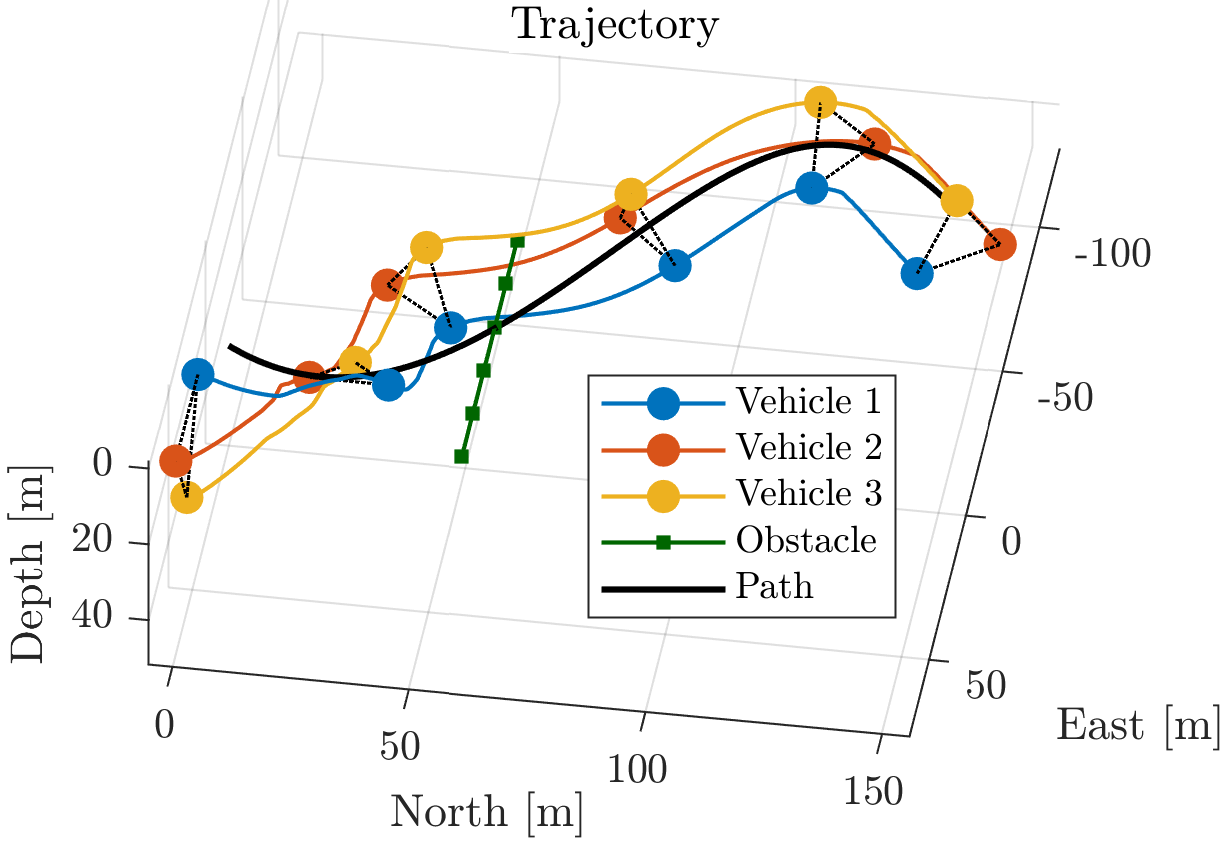
\includegraphics[width=.75\textwidth]{figures/nsb_R/trajectory.png}
    \vspace{-4mm}
    \caption{The 3D trajectory of the vehicles. The markers represent the position of the vehicles at times $t = 0, 50, \ldots, 250$ seconds. Markers with corresponding times are connected by dotted lines to better illustrate the resulting formation.}
    \label{fig:NSB_R_trajectory}
\end{figure}

\pgfplotsset{table/search path={figures/nsb_R/data}}
\begin{figure}[p]
    \centering
    \begin{subfigure}[t]{0.475\textwidth}
        \centering
        % This file was created by matlab2tikz.
%
%The latest updates can be retrieved from
%  http://www.mathworks.com/matlabcentral/fileexchange/22022-matlab2tikz-matlab2tikz
%where you can also make suggestions and rate matlab2tikz.
%
\definecolor{mycolor1}{RGB}{27,158,119}%
\definecolor{mycolor2}{RGB}{233,95,2}%
\definecolor{mycolor3}{RGB}{117,111,179}%
\definecolor{mycolor4}{rgb}{0.50000,1.00000,1.00000}%
%
\begin{tikzpicture}

\begin{axis}[%
width=0.8\textwidth,
height=30mm,
at={(0mm, 0mm)},
scale only axis,
xmin=0,
xmax=250,
xlabel style={font=\color{white!15!black}, yshift=1mm},
xlabel={Time [s]},
xtick={0,50,100,150,200,250},
ymin=0,
ymax=25,
ylabel style={font=\color{white!15!black}},
ylabel={Distance [m]},
axis background/.style={fill=white},
title style={font=\bfseries, yshift=-2.5mm},
title={Smallest distances},
legend style={at={(1.02,0.02)}, anchor=south east, legend cell align=left, align=left, draw=white!15!black, legend columns=2, font=\small}
]
\addplot [color=mycolor1, line width=1pt]
  table[]{simout-1.tsv};
\addlegendentry{Inter-vehicle}

\addplot [color=mycolor2, line width=1pt]
  table[]{simout-2.tsv};
\addlegendentry{Obstacle}

\addplot [color=black, dashed, line width=1.2pt]
  table[]{simout-3.tsv};
\addlegendentry{$d_{\rm COLAV} = r_o$}

\end{axis}
\end{tikzpicture}%

        \vspace{-8mm}
        \caption{The smallest inter-vehicle and vehicle-to-obstacle distance.}
        \label{fig:NSB_R_distances}
        \vspace{-1mm}
    \end{subfigure}
    \hspace{1em}
    \begin{subfigure}[t]{0.475\textwidth}
        \centering
        \hspace*{-1em}
        % This file was created by matlab2tikz.
%
%The latest updates can be retrieved from
%  http://www.mathworks.com/matlabcentral/fileexchange/22022-matlab2tikz-matlab2tikz
%where you can also make suggestions and rate matlab2tikz.
%
\definecolor{mycolor1}{RGB}{27,158,119}%
\definecolor{mycolor2}{RGB}{233,95,2}%
\definecolor{mycolor3}{RGB}{117,111,179}%
\definecolor{mycolor4}{rgb}{0.50000,1.00000,1.00000}%
%
\begin{tikzpicture}

\begin{axis}[%
width=0.8\textwidth,
height=30mm,
at={(0mm, 0mm)},
scale only axis,
xmin=0,
xmax=250,
xlabel style={font=\color{white!15!black}, yshift=1mm},
xlabel={$t$ [s]},
xtick={0,50,100,150,200,250},
y dir=reverse,
ymin=0,
ymax=60,
ylabel style={font=\color{white!15!black}, yshift=-1mm},
ylabel={$z$-coordinate [m]},
axis background/.style={fill=white},
title style={font=\bfseries, yshift=-2.5mm},
title={Depth},
legend style={at={(0.03,0.95)}, anchor=north west, legend cell align=left, align=left, draw=white!15!black, font=\small}
]
\addplot [color=mycolor1, line width=1pt]
    table[]{simout-4.tsv};
\addlegendentry{Smallest depth}

\addplot [color=mycolor2, line width=1pt]
    table[]{simout-5.tsv};
\addlegendentry{Largest depth}

\addplot [color=black, dashed, line width=1.2pt]
    table[]{simout-6.tsv};
\addlegendentry{Depth limits}

\addplot [color=black, dashed, forget plot, line width=1.2pt]
    table[]{simout-7.tsv};
\end{axis}
\end{tikzpicture}

        \vspace{-8mm}
        \caption{The smallest and largest vehicle depth.}
        \label{fig:NSB_R_depth}
        \vspace{-1mm}
    \end{subfigure}
    \begin{subfigure}[t]{0.475\textwidth}
        \centering
        % This file was created by matlab2tikz.
%
%The latest updates can be retrieved from
%  http://www.mathworks.com/matlabcentral/fileexchange/22022-matlab2tikz-matlab2tikz
%where you can also make suggestions and rate matlab2tikz.
%
\definecolor{mycolor1}{RGB}{27,158,119}%
\definecolor{mycolor2}{RGB}{233,95,2}%
\definecolor{mycolor3}{RGB}{117,111,179}%
\definecolor{mycolor4}{rgb}{0.50000,1.00000,1.00000}%
%
\begin{tikzpicture}

\begin{axis}[%
width=0.8\textwidth,
height=25mm,
at={(0mm, 0mm)},
scale only axis,
xmin=0,
xmax=250,
xlabel style={font=\color{white!15!black}, yshift=1mm},
xtick={0,50,100,150,200,250},
xlabel={Time [s]},
ymin=-20.4602266733107,
ymax=24.5,
ylabel style={font=\color{white!15!black}, yshift=-2mm},
ylabel={Error [m]},
axis background/.style={fill=white},
title style={font=\bfseries, yshift=-2.5mm},
title={Path following error},
legend style={at={(0.95,1.)}, anchor=north east, legend cell align=left, align=left, draw=white!15!black, font=\small}
]
\addplot [color=mycolor1, line width=1pt]
    table[]{simout-8.tsv};
\addlegendentry{$x$-error}

\addplot [color=mycolor2, line width=1pt]
    table[]{simout-9.tsv};
\addlegendentry{$y$-error}

\addplot [color=mycolor3, line width=1pt]
    table[]{simout-10.tsv};
\addlegendentry{$z$-error}


\addplot[area legend, dashed, draw=black, fill=green, fill opacity=0.15, forget plot]
table[] {simout-11.tsv}--cycle;

\addplot[area legend, dashed, draw=black, fill=orange, fill opacity=0.15, forget plot]
table[] {simout-12.tsv}--cycle;

\addplot[area legend, dashed, draw=black, fill=orange, fill opacity=0.15, forget plot]
table[] {simout-13.tsv}--cycle;
\end{axis}
\end{tikzpicture}

        \vspace{-8mm}
        \caption{The path-following error. The green rectangle represents the time when obstacle avoidance is active. The red rectangle represents the time when depth limiting is active.}
        \label{fig:NSB_R_path_following_error}
        \vspace{-1mm}
    \end{subfigure}
    \hspace{1em}
    \begin{subfigure}[t]{0.475\textwidth}
        \centering
        \hspace*{-1.1em}
        % This file was created by matlab2tikz.
%
%The latest updates can be retrieved from
%  http://www.mathworks.com/matlabcentral/fileexchange/22022-matlab2tikz-matlab2tikz
%where you can also make suggestions and rate matlab2tikz.
%
\definecolor{mycolor1}{RGB}{27,158,119}%
\definecolor{mycolor2}{RGB}{233,95,2}%
\definecolor{mycolor3}{RGB}{117,111,179}%
\definecolor{mycolor4}{rgb}{0.50000,1.00000,1.00000}%
%
\begin{tikzpicture}

\begin{axis}[%
width=0.8\textwidth,
height=25mm,
at={(0mm, 0mm)},
scale only axis,
xmin=0,
xmax=250,
xlabel style={font=\color{white!15!black}, yshift=1mm},
xlabel={$t$ [s]},
xtick={0,50,100,150,200,250},
ymin=-25,
ymax=25,
ylabel style={font=\color{white!15!black}, yshift=-3.5mm},
ylabel={Error [m]},
axis background/.style={fill=white},
title style={font=\bfseries, yshift=-2.5mm},
title={Formation keeping error},
legend style={at={(0.97,0.03)}, anchor=south east, legend cell align=left, align=left, draw=white!15!black, legend columns=1, font=\small}
]
\addplot [color=mycolor1, line width=1pt]
    table[]{simout-14.tsv};
    \addlegendentry{$ x$ [m]}
\addplot [color=mycolor1, dashed, forget plot, line width=1.1pt]
    table[]{simout-15.tsv};
\addplot [color=mycolor1, dotted, forget plot, line width=1.3pt]
    table[]{simout-16.tsv};
\addplot [color=mycolor2, line width=1pt]
    table[]{simout-17.tsv};
    \addlegendentry{$ y$ [m]}
\addplot [color=mycolor2, dashed, forget plot, line width=1.1pt]
    table[]{simout-18.tsv};
\addplot [color=mycolor2, dotted, forget plot, line width=1.3pt]
    table[]{simout-19.tsv};
\addplot [color=mycolor3, line width=1pt]
    table[]{simout-20.tsv};
    \addlegendentry{$ z$ [m]}
\addplot [color=mycolor3, dashed, forget plot, line width=1.1pt]
    table[]{simout-21.tsv};
\addplot [color=mycolor3, dotted, forget plot, line width=1.3pt]
    table[]{simout-22.tsv};

\addplot[area legend, dashed, draw=black, fill=mycolor4, fill opacity=0.25, forget plot]
table[] {simout-23.tsv}--cycle;
\end{axis}

\end{tikzpicture}
        \vspace{-8mm}
        \caption{The formation-keeping error. The full, dashed, and dotted lines correspond to vehicles 1, 2, and 3, respectively. The blue rectangle represents the time when inter-agent \gls{colav} is active.}
        \label{fig:NSB_R_formation_keeping_error}
        \vspace{-1mm}
    \end{subfigure}
    \begin{subfigure}[t]{0.475\textwidth}
        \centering
        % This file was created by matlab2tikz.
%
%The latest updates can be retrieved from
%  http://www.mathworks.com/matlabcentral/fileexchange/22022-matlab2tikz-matlab2tikz
%where you can also make suggestions and rate matlab2tikz.
%
\definecolor{mycolor1}{RGB}{27,158,119}%
\definecolor{mycolor2}{RGB}{233,95,2}%
\definecolor{mycolor3}{RGB}{117,111,179}%
\definecolor{mycolor4}{rgb}{0.50000,1.00000,1.00000}%
%
\begin{tikzpicture}

\begin{axis}[%
width=0.8\textwidth,
height=25mm,
at={(0mm, 0mm)},
scale only axis,
xmin=0,
xmax=250,
xlabel style={font=\color{white!15!black}, yshift=1mm},
xlabel={$t$ [s]},
xtick={0,50,100,150,200,250},
ymin=0,
ymax=1.4,
ylabel style={font=\color{white!15!black}, yshift=-2mm},
ylabel={Velocity [m/s]},
axis background/.style={fill=white},
title style={font=\bfseries, yshift=-2.5mm},
title={Surge velocity},
legend style={at={(0.97,0.07)}, anchor=south east, legend cell align=left, align=left, draw=white!15!black, legend columns=4, font=\small}
]
\addplot [color=mycolor1, line width=1pt]
  table[]{states-1.tsv};
  \addlegendentry{$u_1$}
\addplot [color=mycolor2, line width=1pt]
  table[]{states-2.tsv};
  \addlegendentry{$u_3$}
\addplot [color=mycolor3, line width=1pt]
  table[]{states-3.tsv};
  \addlegendentry{$u_2$}
\addplot [color=black, dashed, line width=1.2pt]
  table[]{states-10.tsv};
  \addlegendentry{$u_{\min}$}

\addplot[area legend, dotted, draw=black, fill=gray, fill opacity=0.15, forget plot]
table[] {states-11.tsv}--cycle;

\addplot[area legend, dotted, draw=black, fill=gray, fill opacity=0.15, forget plot]
table[] {states-12.tsv}--cycle;
\end{axis}
\end{tikzpicture}

        \vspace{-8mm}
        \caption{The surge velocities of the vehicles. The grey rectangle represents the time when any avoidance task is active.}
        \label{fig:NSB_R_surge}
        \vspace{-2.5mm}
    \end{subfigure}
    \hspace{1em}
    \begin{subfigure}[t]{0.475\textwidth}
        \centering
        \hspace*{-1.3em}
        % This file was created by matlab2tikz.
%
%The latest updates can be retrieved from
%  http://www.mathworks.com/matlabcentral/fileexchange/22022-matlab2tikz-matlab2tikz
%where you can also make suggestions and rate matlab2tikz.
%
\definecolor{mycolor1}{RGB}{27,158,119}%
\definecolor{mycolor2}{RGB}{233,95,2}%
\definecolor{mycolor3}{RGB}{117,111,179}%
\definecolor{mycolor4}{rgb}{0.50000,1.00000,1.00000}%
%
\begin{tikzpicture}

\begin{axis}[%
width=0.8\textwidth,
height=25mm,
at={(0mm, 0mm)},
scale only axis,
xmin=0,
xmax=250,
xlabel style={font=\color{white!15!black}, yshift=1mm},
xlabel={Time [s]},
xtick={0,50,100,150,200,250},
ymin=-0.1,
ymax=0.2,
ylabel style={font=\color{white!15!black}, yshift=-4mm},
ylabel={Velocity [m/s]},
axis background/.style={fill=white},
title style={font=\bfseries, yshift=-2.5mm},
title={Underactuated dynamics},
legend style={at={(0.97,0.05)}, anchor=south east, legend cell align=left, align=left, draw=white!15!black, legend columns=3, font=\small}
]
\addplot [color=mycolor1, line width=1pt]
  table[]{states-4.tsv};
  \addlegendentry{$v$}
\addplot [color=mycolor1, dashed, forget plot, line width=1.1pt]
  table[]{states-5.tsv};  
\addplot [color=mycolor1, dotted, forget plot, line width=1.3pt]
  table[]{states-6.tsv}; 

\addplot [color=mycolor2, line width=1pt]
  table[]{states-7.tsv};
  \addlegendentry{$w$}
\addplot [color=mycolor2, dashed, forget plot, line width=1.1pt]
  table[]{states-8.tsv};  
\addplot [color=mycolor2, dotted, forget plot, line width=1.3pt]
  table[]{states-9.tsv}; 

\addplot[area legend, dotted, draw=black, fill=gray, fill opacity=0.15, forget plot]
  table[] {states-22.tsv}--cycle;  
\addplot[area legend, dotted, draw=black, fill=gray, fill opacity=0.15, forget plot]
  table[] {states-23.tsv}--cycle;
\end{axis}

\end{tikzpicture}

        \vspace{-8mm}
        \caption{The sway and heave velocities. The full, dashed, and dotted lines correspond to vehicles 1, 2, and 3, respectively.}
        \label{fig:NSB_R_sway_heave}
        \vspace{-2.5mm}
    \end{subfigure}
    \caption{Simulation results.}
    \label{fig:NSB_R_results}    
\end{figure}

The very minimum relative distance to avoid collision is the length of the \gls{lauv}, \emph{i.e.}, $2.4$ m.
For additional safety, we design the \gls{colav} task with $d_{\rm min} = 5$ m.
For additional safety during transients, $d_{\rm COLAV}$ is chosen to be $10$ m.



We then let the vehicles encounter an obstacle of similar size as the \gls{lauv} that moves east at a constant speed of $\SI{0.3}{\meter\per\second}$.
Given its size, we choose $r_o = d_{\rm COLAV}$.
The minimum cone angle is set to $\alpha_{\min} = \SI{15}{\degree}$.
The operation limits are chosen as $z_{\min} = \SI{1}{m}$, $z_{\max} = \SI{49}{m}$, and the depth-limiting velocity is $\ivels_z = \SI{0.3}{\meter\per\second}$.
Note that the limits are deliberately chosen too small for the given path and formation, so that depth limiting is activated.



Figures \ref{fig:NSB_R_trajectory} and \ref{fig:NSB_R_results} show the results of this numerical simulation.
%The initial conditions are chosen identically as in \cite{matouvs_formation_2022}, so that we can directly compare the results.
\figref{fig:NSB_R_distances} shows the distance between the vehicles and the distance to the obstacle.
At $t = \SI{20}{\second}$, the \gls{colav} task is activated, and the distance between the vehicles drops to approximately $9.5$ meters during the transient.
The situation is resolved after $30$ seconds.
At $t = \SI{35}{\second}$, the vehicles enter the collision cone and perform an evasive maneuver in a clockwise direction.
The distance to the obstacle is always above the required limit.



\figref{fig:NSB_R_depth} shows the depth of the vehicles.
At $t = \SI{73}{\second}$ and $t = \SI{212}{\second}$, the depth-limiting task is activated.
When the task is active, the depth of the vehicles fluctuates around the prescribed limit.



Figures \ref{fig:NSB_R_path_following_error} and \ref{fig:NSB_R_formation_keeping_error} show the path-following and formation-keeping errors.
We can see that the path-following errors diverge when obstacle avoidance or depth limiting is active.
Conversely, the formation-keeping errors diverge during inter-agent \gls{colav}.
This behavior corresponds to the interpretation of the \gls{nsb} tasks --- path-following is global and thus cannot be satisfied during obstacle avoidance, whereas formation-keeping works with relative velocities and thus cannot be satisfied during inter-agent \gls{colav}.



\figref{fig:NSB_R_surge} shows the surge velocity of the vehicles.
We can see that the surge velocities are always above the required limit.
In fact, our solution appears to be overly conservative.
\figref{fig:NSB_R_sway_heave} shows the sway and heave velocities.
We can see that the velocities change abruptly when the collision avoidance or depth limiting tasks are active, as the vehicles switch to a different behavior.
However, the velocities still remain bounded during the whole simulation.
The peak in sway velocities at $t = \SI{180}{\second}$ coincides with the sharpest turn (\emph{i.e.,} the largest $\bs{\omega}_p(s)$) of the desired path.
